% LaTeX formatting example for NERCCS
% Revised on 8/23/2018 by Hiroki Sayama

\documentclass[12pt]{article}
\usepackage[letterpaper,margin=1in]{geometry}
\usepackage{times}
\usepackage{graphicx}
\usepackage{sectsty}
\allsectionsfont{\normalsize}
\usepackage{authblk}
\renewcommand\Authfont{\normalsize}

\begin{document}

\title{\normalsize\bf%
The Specialization Model for Network Growth}

\author{L. A. Bunimovich$^1$, D. Passey$^2$, D. Smith$^2$, and B. Webb$^2$,\\
$^1$ Georgia Institute of Technology\\
bunimovh@math.gatech.edu\\
$^2$ Brigham Young University\\
dj@math.byu.edu, dallas.smith@math.byu.edu, bwebb@math.byu.edu\\}

\date{\vspace{-5ex}} % to kill the unnecessary blank space for \date{}

\maketitle

\thispagestyle{empty}
\pagestyle{empty}


\begin{abstract}\normalsize
Dynamics in many real world complex networks exhibit a robustness to perturbations that is difficult to model. The difficulty arises when attempts are made to reproduce highly modular and hierarchical structure while also maintaining stability.

We introduce the specialization model of network growth to address this issue. As real world networks grow, sub-networks become specialized in preforming specific tasks. Our model mimics this behavior by maintaining and replicating the components of a network as it grows.

The specialization of a network via our process preserves spectral radius associated with the network's adjacency matrix. This allows us to show that a network maintains certain dynamic properties, specifically stability under mild conditions, as the network's topology becomes increasingly complex due to specialization.

Our specialized networks exhibit the desired increases in modularity, sparsity and hierarchical structure found in gene regulatory networks, the brain and the internet. Networks generated using our model also demonstrate many well known properties of real-wold networks such as the small-world property, disassortativity, power-law like degree distributions and clustering coefficients.

In addition to stability, specialization allows us to grow isolated components of the network. Using eigenvector centrality as a metric, we describe how the importance of these components evolves as they are specialized. Together these two ideas allow us to preserve the importance of some areas in the network while adjusting the importance of other areas in a structured way.


\end{abstract}

\begin{figure}[h]
\centering
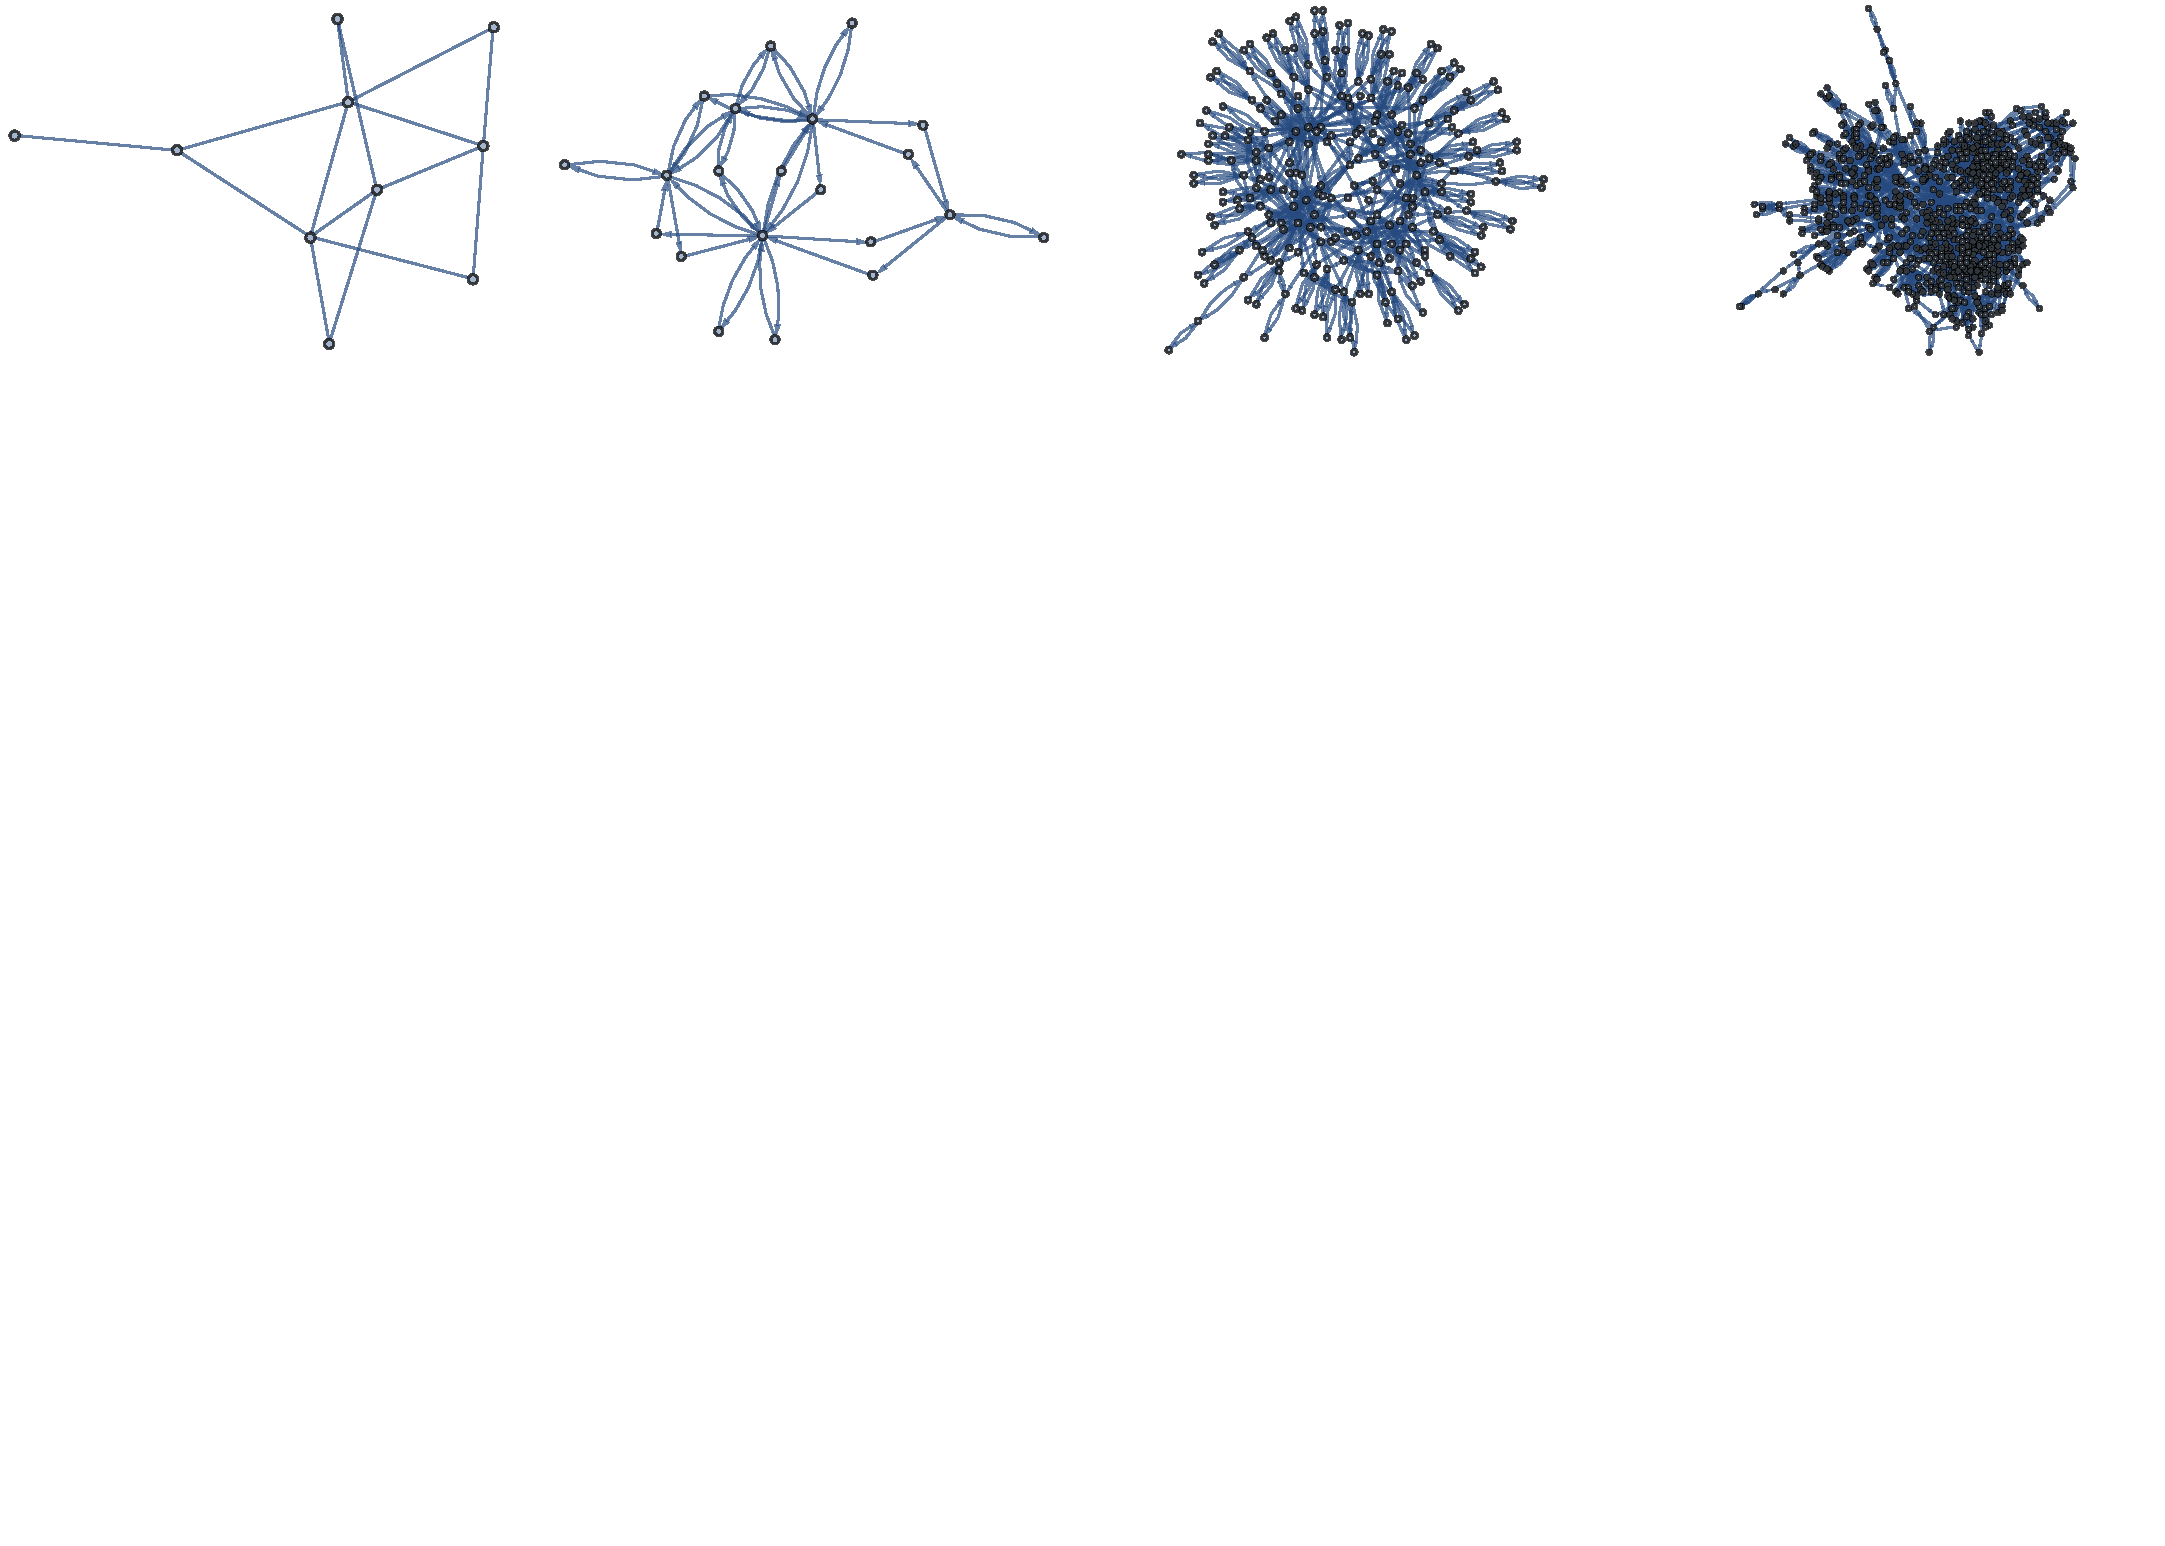
\includegraphics[width=0.6\columnwidth]{specfig.pdf}
\caption{The stages of a network grown via the specialization model. The adjacency matrix of each network pictured has the same spectral radius.}
\label{fig:sinx}
\end{figure}



\end{document}